\chapter{Einleitung}

\section{Motivation und Problemstellung}

Die digitale Transformation hat tiefgreifende Auswirkungen auf das private und geschäftliche Umfeld und stellt damit auch die eher träge auf Veränderungen reagierende deutsche Versicherungsindustrie vor neue Herausforderungen. Der Wettbewerb in der Branche verschärft sich und Kunden fordern fortlaufend bessere Serviceangebote und -qualität. Moderne, wechselwillige Kunden möchten mit ihrem Versicherer auf Self-Service-Basis interagieren, um Angebote zu erhalten, Anträge zu stellen oder Ansprüche geltend zu machen. \autocite[Vgl.][]{SCHMIDT2022}

Besonders deutlich sind diese Veränderungen in der Kraftfahrzeug-Versicherungs-branche (\acsu{kfz}-Versicherungsbranche) zu erkennen. So ist gemäß einer Studie von Statista aus dem Jahr 2022 die \ac{kfz}-Versicherungssparte mit mehr als 26\% online abgeschlossener Verträge in der deutschen Versicherungsindustrie aktuell führend. \autocite[Vgl.][]{STATISTA2023} Bei der Wahl des Anbieters stehen dabei vor allem die Einfachheit und Klarheit der Versicherungsleistung, die Anpassungsmöglichkeiten an das Fahrverhalten sowie der Preis im Vordergrund. \autocite[Vgl.][]{MITZNER2023} 

Folglich müssen \ac{kfz}-Versicherer ihre internen Prozesse zur Kostenreduktion optimieren und ihren digitalen Auftritt verbessern, um langfristig am Markt wettbewerbsfähig zu sein bzw. zu bleiben. Für diese digitale Transformation ist dabei nicht eine einzelne Komponente entscheidend, sondern benötigen die \ac{kfz}-Versicherer vielmehr eine digitale Plattform, mit der sie eine durchgehende Digitalisierung, Optimierung interner Prozesse sowie eine intelligente Datennutzung erreichen können. \autocite[Vgl.][]{WEINGARTNER2023} 

%\newpage
\section{Zielsetzung und Abgrenzung}

Die SAP \ac{btp} ist eine digitale Plattform, mit der \ac{kfz}-Versicherer ihre bestehende Systemlandschaft transformieren und an neue Geschäftsanforderungen anpassen können.

Ziel dieser Arbeit ist es daher, die Anforderungen der \ac{kfz}-Versicherer an eine digitale Plattform zu identifizieren, um anschließend beurteilen zu können, inwiefern die Anforderungen der \ac{kfz}-Versicherer an eine digitale Plattform von der SAP Business Technology Plattform erfüllt werden. Die aus der Analyse resultierende Handlungsempfehlung soll \ac{kfz}-Versicherern eine praxisorientierte Vorgehensweise zur Nutzung der SAP Business Technology Plattform aufzeigen.

\improvement{Muss ich hier aus dem Inwiefern nicht nochmal ein ob machen?}
Dabei wird der deutsche \ac{kfz}-Versicherungsmarkt betrachtet, da eine Analyse inklusive internationaler Märkte aufgrund der unterschiedlichen regulatorischen Rahmenbedingungen, divergierender Prämienfaktoren sowie ungleichmäßig ausgeprägter technologischer Fortschritte nicht hinreichend aussagekräftig wäre. Des Weiteren konzentriert sich die Arbeit im Wesentlichen auf die technologischen Merkmale einer digitalen Plattform. Darüber hinaus werden im Rahmen dieser Untersuchung digitaler Plattformen als Wettbewerbsfaktor betrachtet, nicht aber in Bezug zu anderen Wettbewerbskräften im Versicherungsmarkt gesetzt.




\section{Aufbau der Arbeit}

Zu Beginn der Projektarbeit werden zunächst digitale Plattformen als disruptive Innovation erläutert. Hierzu werden digitale Plattformen definiert, die Wertschöpfung digitaler Plattformen vorgestellt, Cloud-Computing auf technischen Plattformen beschrieben und darauf aufbauend die SAP Business Technology Platform vorgestellt. Danach werden die Definition und Grundprinzipien der Versicherung sowie der Aufbau und der Wettbewerb in der \ac{kfz}-Versicherungssparte dargestellt. Anschließend wird die Wahl der wissenschaftlichen Methodik begründet und das Vorgehen bei der Task-Technology-Fit-Theorie (\acsu{ttf}-Theorie), der systematischen Literaturanalyse, dem semistrukturierten Leitfadeninterview sowie bei der qualitativen Inhaltsanalyse beschrieben. Danach werden die Anforderungen der \ac{kfz}-Versicherer an digitale Plattformen mithilfe der systematischen Literaturanalyse identifiziert und anschließend mittels Experteninterviews ergänzt und evaluiert. Daraufhin werden die Funktionalitäten und Services der SAP \ac{btp} vorgestellt, um diese im Anschluss den Anforderungen der \ac{kfz}-Versicherer gegenüberzustellen. Ausgehend von dem Analyseergebnis wird eine Handlungsempfehlung für deutsche \ac{kfz}-Versicherer ausgesprochen. Darauffolgend werden die Vorgehensweise und Analyseergebnisse kritisch reflektiert, um abschließend die Arbeit mit einem Fazit zusammenzufassen und in einem Ausblick mögliche Folgeuntersuchungen aufzuzeigen.(siehe Abbildung \ref{fig:Aufbau})


\begin{figure}[h]
    \centering
    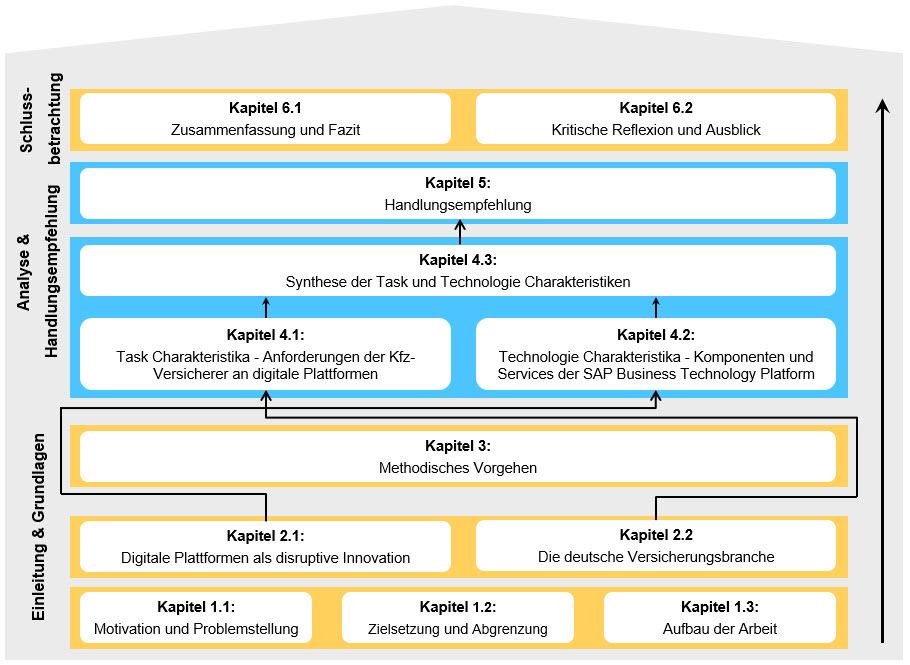
\includegraphics[width=1\textwidth]{img/Aufbau_der_Arbeit2.jpg}
    \caption[Aufbau der Arbeit]{Aufbau der Arbeit\autocite{Aufbau}}
    \label{fig:Aufbau}
\end{figure}
\footnotetext{eigene Darstellung}

\newpage